

To count all the flux in all cluster galaxies, we must make two
corrections: (1) add the galaxy light outside of the MAG\_AUTO
aperture, and (2) add the luminosity of all cluster galaxies below the
detection threshold of our galaxy catalog. We use a Monte Carlo
simulation of galaxies placed on the real survey data to determine
both the detection efficiency as a function of galaxy magnitude, and
the fraction of galaxy light inside the MAG\_AUTO aperture. 

\subsubsection{Galaxy Monte Carlo Simulation}

Each simulated galaxy has an elliptical S{\'e}rsic profile
given by
\begin{equation}
r = \sqrt{x^2 + (y/q)^2}
\end{equation}
\begin{equation}
\Sigma(r) = \Sigma_e e^{-\kappa [(r/r_e)^{1/n}-1]}
\end{equation}
where $\kappa$ is coupled to $n$ such that half the total flux is
always within $r_e$. For $n \gtrsim 2$, $\kappa \approx 2n - 0.331$;
at low $n$, $\kappa(n)$ flattens out toward 0, and is obtained by
interpolation. Here we use the approximation $\kappa(n)=1.7233
n^{1.0902}$ for $0<n<2$ and $\kappa = 2n -0.331$ for $n>2$. The total
flux is given by
\begin{equation}
F_{\rm tot} = 2\pi r_e^2 \Sigma_e e^\kappa n \kappa^{-2n} \Gamma(2n)q
\end{equation}
\newpage

%%%%%%%%%%%%%%%%%%%%%%%%%%%%%%%%%%%%%%%%%%%%%%%%%%
% FIGURE: ONE SIMULATED GALAXY                   %
%%%%%%%%%%%%%%%%%%%%%%%%%%%%%%%%%%%%%%%%%%%%%%%%%%
\begin{SCfigure}[0.7][tp]
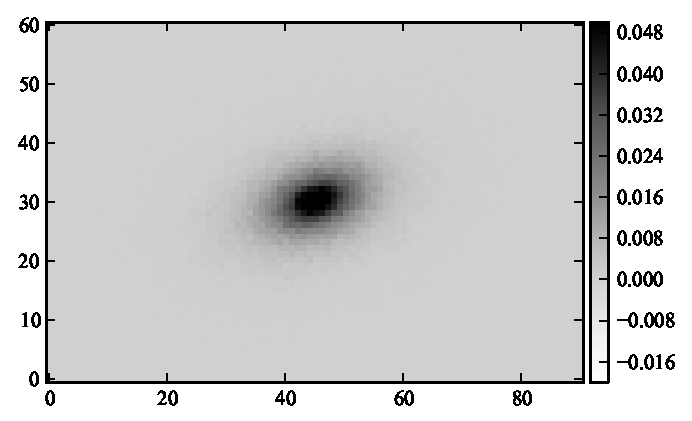
\includegraphics[width=0.65\textwidth]{figures/clrate/onesimgal.eps}
\caption[Example of a simulated galaxy]{Example of a simulated galaxy
with S{\'e}rsic index $n=1$, ellipticity $q=0.6$, magnitude $z_{850} =
  22.5$, and effective radius $r_e = 9$ pixels. Poisson noise is
  included but background noise has not been
  added. \label{fig:onesimgal}}
\end{SCfigure}

%%%%%%%%%%%%%%%%%%%%%%%%%%%%%%%%%%%%%%%%%%%%%%%%%%
% FIGURE: R_E OF SPECTROSCOPIC REDSHIFT GALAXIES %
%%%%%%%%%%%%%%%%%%%%%%%%%%%%%%%%%%%%%%%%%%%%%%%%%%
\begin{figure}[hp]
\begin{center}
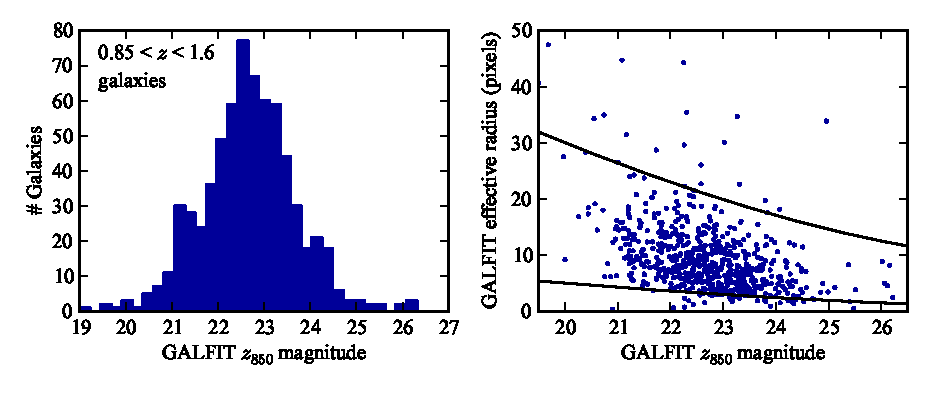
\includegraphics{figures/clrate/specgals.eps}
\end{center}
\caption[Effective radii of spectroscopically-confirmed galaxies]{{\it
    Left panel:} The distribution of GALFIT $z_{850}$ magnitudes for
  the 672 galaxies with spectroscopic redshifts $0.85 < z < 1.6$.
  {\it Right panel:} The GALFIT effective radius $r_e$ as a function
  of magnitude for the same galaxies. The black lines show the range
  of effective radius used in the Monte Carlo. Given a simulated
  galaxy magnitude, an effective radius is randomly selected from a
  flat distribution between the lower and upper black lines.
  \label{fig:specgals}}
\end{figure}

\noindent where $\Gamma(2n)$ is the gamma function. The
simulated galaxy is convolved with a (very rough) $3 \times 3$ PSF and
Poisson noise is added.  Each galaxy is simulated out to a radius of $5r_e$. 
An example of a simulated galaxy is shown in Figure~\ref{fig:onesimgal}.

The S{\'e}rsic index $n$ is simply selected from a flat distribution
ranging from $n = 0.7$ to $n = 4.5$, and the minor to major axis ratio
$q$ selected from a flat distribution ranging from $q = 0.3$ to $q =
1$.  The distribution of galaxy angular sizes $r_e$ will also affect the
results. For guidance on the size of the galaxies of concern (namely,
those at $z \gtrsim 0.9$) we turned to the 672 galaxies in the survey
with spectroscopic redshifts in the range $0.85<z<1.6$. These 672
galaxies were all fit with {\sc galfit} \citep{peng02a}, which fits a
value for $r_e$.  Figure~\ref{fig:specgals} (left panel) shows the
distribution of $r_e$ and total magnitude for these galaxies. Based on
this distribution (and considering that dimmer galaxies and those with
larger effective radii are selected against), we chose a range of
effective radius that depends on the magnitude, shown in
Fig.~\ref{fig:specgals}, left panel, between the two black
lines. Given a magnitude, a galaxy's effective radius is chosen from a
uniform distribution of $r_e$ in the range shown.

\begin{figure}[t]
\begin{center}
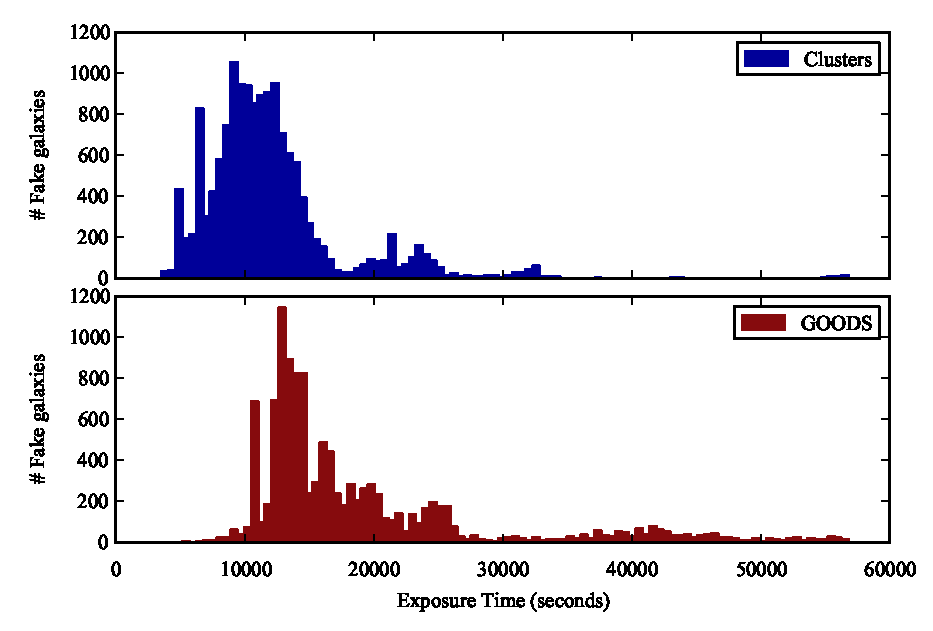
\includegraphics{figures/clrate/fakegals_exptime.eps}
\end{center}
\caption[Image depths at location of simulated galaxies]{The
  distribution of image depths (in effective exposure time) at the
  location of simulated galaxies. {\it Top panel:} A total of 15,000
  simulated galaxies were placed on cluster images. {\it Bottom
    panel:} A total of 12,000 simulated galaxies were placed on GOODS
  images. 304 galaxies were placed on the HUDF which has an effective
  exposure time of approximately 350,000 seconds, and are thus not
  shown.\label{fig:exptime}}
\end{figure}

To avoid overcrowding the images, only 200 galaxies are placed on each
image. Galaxies are only placed on the same regions of the images used
in the cluster luminosity analysis. For the GOODS fields, this is
selected circular regions with radii 1.4~arcminutes. For the cluster
fields, only regions with effective exposure time above a certain
threshold are used. This effectively eliminates the outskirts of each
field, leaving a region with mostly uniform depth for each
cluster. The distribution of effective exposure times at the location
of the simulated galaxies is shown in Fig.~\ref{fig:exptime} for all
galaxies placed on cluster fields (top panel) and all galaxies placed
on GOODS fields (bottom panel). Additionally, we enforce a minimum
separation of 10 pixels between the center of a simulated galaxy and
the center of any existing galaxy (and a minimum separation of 100
pixels from the center of any existing galaxy brighter than
$z_{850} \sim 21$). This ensures that the simulated galaxies will not
be confused with existing galaxies and the output catalog will be
cleanly comparable with the input catalog. A total of 15,000 and
12,000 galaxies were simulated on cluster fields and GOODS fields
respectively.

Images with simulated galaxies added are then run through the
background-subtraction and catalog-extraction pipelines. The resulting
catalog for each image is then compared to the input galaxies. The
closest detected galaxy within 5 pixels of a simulated galaxy is
matched to the simulated galaxy. If no galaxy is detected within 5
pixels of a simulated galaxy, the galaxy is counted as not having been
found by {\sc SExtractor}. 

\subsubsection{Galaxy Detection Efficiency}

%%%%%%%%%%%%%%%%%%%%%%%%%%%%%%%%%%%%%%%
% FIGURE: GALAXY DETECTION EFFICIENCY %
%%%%%%%%%%%%%%%%%%%%%%%%%%%%%%%%%%%%%%%
\begin{figure}[tp]
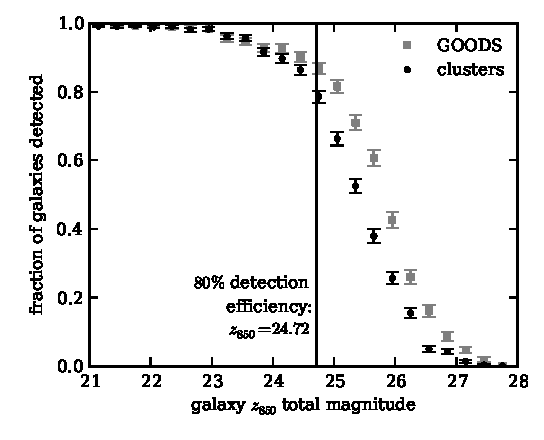
\includegraphics[width=0.5\textwidth]{figures/clrate/fakegals_eff.eps}
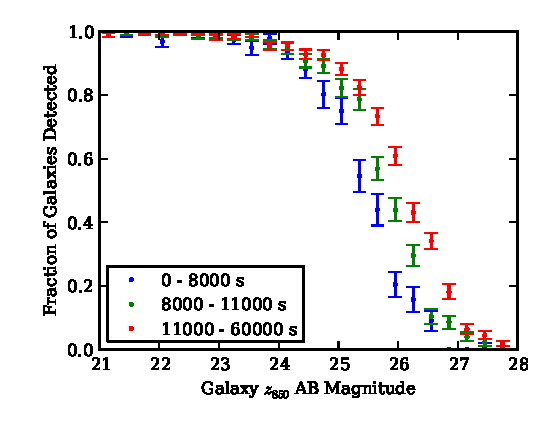
\includegraphics[width=0.5\textwidth]{figures/clrate/fakegals_eff_exptime.eps}
\caption[Simulated galaxy detection efficiency]{{\it Left panel:} Percentage of simulated 
galaxies recovered by {\sc SExtractor} as a function of total galaxy
  $z_{850}$ magnitude for simulated galaxies placed on cluster fields
  (black circles) and GOODS fields (grey squares). The
  detection efficiency drops to 80\% at $z_{850} = 24.72$ for cluster
  fields (vertical line). We discard all galaxies dimmer than
  this value.  {\it Right panel:} The variation in detection
  efficiency with exposure time, for cluster fields only.  There are
  2654, 4877, and 7469 galaxies in the three bins in order of
  increasing image depth. The corresponding 80\% recovery magnitudes
  are 24.76, 25.33, and 25.48 (AB). The differences in detection
  efficiency are small, particularly above the $z_{850}$ = 24.72 (Vega) =
  25.26 (AB) magnitude cutoff.
\label{fig:fakegals_eff}}
\end{figure}

The detection efficiency as a function of galaxy magnitude is shown in
Figure~\ref{fig:fakegals_eff}. For the average of all cluster fields,
the detection efficiency drops to 80\% at $z_{850} = 24.72$. We use
this magnitude as a cutoff in our selection, discarding all galaxies
dimmer than this magnitude.  We later correct total cluster
luminosities for the uncounted light from these galaxies by using an
assumed cluster luminosity function.  In reality, the detection
efficiency varies slightly from field to field (and even within a
field) due to exposure time variations (Fig.~\ref{fig:fakegals_eff},
right panel, shows the variation in detection efficiency with exposure
time for cluster fields). However, to first order the variation is
accounted for by using the average efficiency in all fields. In
addition, the total luminosity of $z_{850} > 24.72$ cluster galaxies
is small (as shown below), so slight changes in the cutoff will have a
negligible effect on the total luminosity.

\subsubsection{MAG\_AUTO Aperture Correction}

%%%%%%%%%%%%%%%%%%%%%%%%%%%%%%%%%%%%%%%%%%%%%%%%%%%%%%%%%%%%%%%%%%
% PLOT: GALAXY MAG_AUTO CORRECTION : PAGE GRID of N vs Delta Mag %
%%%%%%%%%%%%%%%%%%%%%%%%%%%%%%%%%%%%%%%%%%%%%%%%%%%%%%%%%%%%%%%%%%
\begin{figure}[tp]
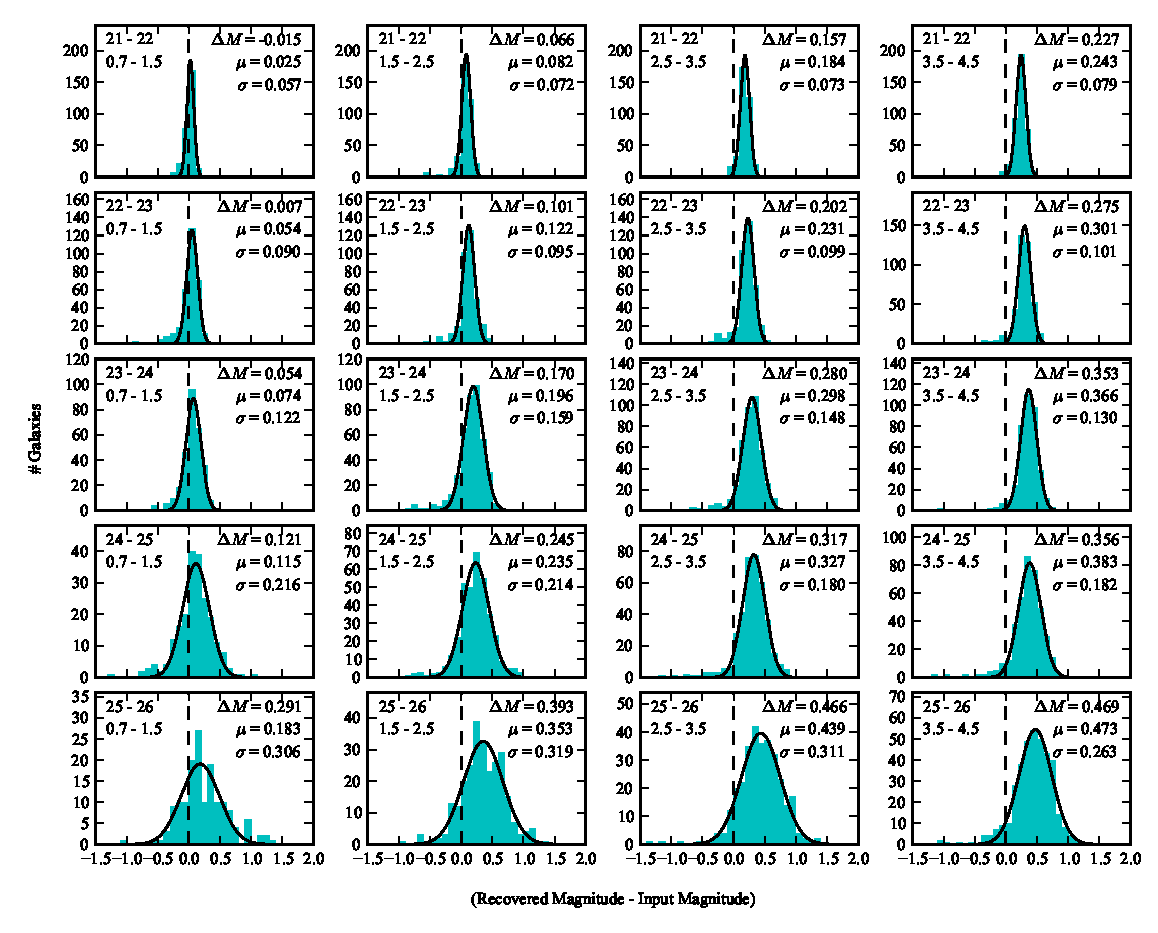
\includegraphics[angle=270]{figures/clrate/fakegals_grid_n.eps}
\caption[Aperture correction as a function of magnitude and S{\'e}rsic
index $n$]{The distribution of aperture corrections as a function of
magnitude and S{\'e}rsic index $n$. The range of magnitudes and
S{\'e}rsic indices included in each panel is given in the upper left
of the panel. $\Delta M$ is the magnitude correction derived from
ratio of the total flux extracted to the total flux input. $\mu$ and
$\sigma$ describe the Gaussian fit to each distribution. 
\label{fig:fakegals_grid_n}}
\end{figure}

The fraction of galaxy light falling inside the MAG\_AUTO aperture
will depend on several parameters of the galaxy, including the galaxy
magnitude, and S{\'e}rsic index $n$. To see the dependence on
magnitude and $n$, in Figure~\ref{fig:fakegals_grid_n} we split the
simulated galaxies into bins in magnitude and $n$. For the galaxies in
each bin, we plot the distribution of the difference between the true
total magnitude and the MAG\_AUTO magnitude.  A Gaussian fit, and its
$\mu$ and $\sigma$ parameters, are shown for reference. As expected,
the distributions are wider for fainter magnitudes (descending rows in
the figure) due to increasing photometric error. The distributions
have somewhat non-Gaussian tails, particularly on the negative side. On
the negative side, this is most likely due to collisions with other
galaxies, where flux from a nearby galaxy falls in the aperture. Also
as expected, the offset grows larger with both increasing $n$ and
increasing magnitude. As $n$ or magnitude increases, the outskirts of
the galaxy are increasingly buried in noise, causing {\sc SExtractor}
to underestimate the Kron radius, leading to a smaller MAG\_AUTO
aperture.  For each distribution, $\Delta M$ is the magnitude
correction one would need to make to each galaxy in order for
the \emph{total} output flux to match the \emph{total} input
flux. Aperture corrections are based on $\Delta M$ in each bin, and
thus take into account the non-Gaussian tails in the distributions.


%%%%%%%%%%%%%%%%%%%%%%%%%%%%%%%%%%%%
% PLOT: GALAXY MAG_AUTO CORRECTION %
%%%%%%%%%%%%%%%%%%%%%%%%%%%%%%%%%%%%
\begin{SCfigure}[0.7][tb]
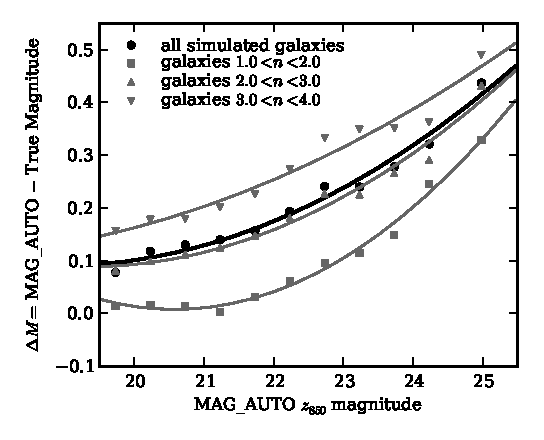
\includegraphics[width=0.6\textwidth]{figures/clrate/fakegals_apcorr.eps}
\caption[Aperture correction as a function of magnitude]{Galaxy 
MAG\_AUTO aperture correction as a function of galaxy magnitude. The
black circles show the average correction for the full distribution of
galaxies simulated, including all S{\'e}rsic indices $n$. The black
line is a fit to these points and is the relation we use. Note that it
is not extrapolated beyond the range shown. To illustrate the effect
of $n$ on the aperture correction, we plot the aperture correction for
subsets of galaxies with different S{\'e}rsic indices (Grey
squares and triangles). Galaxies with larger S{\'e}rsic indices have
a larger aperture correction.
\label{fig:fakegals_apcorr}}
\end{SCfigure}

We derive a relation between $\Delta M$ and the galaxy brightness
(Fig.~\ref{fig:fakegals_apcorr}, black circles), summing over all
$n$. We find that the relation is well-fit by a second-order
polynomial (Fig.~\ref{fig:fakegals_apcorr}, thick black line), given
by
\begin{equation}
\Delta M = 0.238 + 0.081(M_{MAG\_AUTO}-23) + 0.009(M_{MAG\_AUTO} -23)^2.
\end{equation}
%\begin{eqnarray}
%\Delta M & = & 0.238 + 0.081(M_{MAG\_AUTO}-23) + \nonumber \\
%         &   & + 0.009(M_{MAG\_AUTO} -23)^2.
%\end{eqnarray}
We use this to correct the magnitude of each detected galaxy. Note
that the correction is not extrapolated beyond the fitted range shown.

Because we cannot reliably determine $r_e$ or the S{\'e}rsic index $n$
for each galaxy, we rely on the simulated distribution of $r_e$ and
$n$ to accurately represent the true distributions. (The black circles
in Fig.~\ref{fig:fakegals_apcorr} include all simulated galaxies.)  We
have based our distribution of $r_e$ on actual galaxies, but $n$ is
less well-known. To estimate the effect of varying the $n$
distribution, we show $\Delta M$ for subsets of the simulated
galaxies, divided by S{\'e}rsic index (Fig.~\ref{fig:fakegals_apcorr},
grey points and lines).  If, instead of the flat $1<n<4$ distribution
used, all galaxies had $1<n<2$, the aperture correction would be lower
by approximately 0.10~magnitudes. If instead all galaxies had
$3<n<4$, the correction would be higher by approximately
$0.07$~magnitudes. We use $0.07$~mag as the systematic uncertainty in
the aperture correction. (All systematic uncertainties are summarized
in \S\ref{sec:clrate_results_sys} and Table~\ref{tab:clrate_sys}.)

\vspace{1in}
